\documentclass{article}

\title{Architecture document}
\date{8-09-2016}
\author{Robert Kraaijeveld}

\usepackage{graphicx}
\usepackage{fancyhdr}
\usepackage{parskip}
\usepackage[]{algorithm2e}

\pagestyle{fancy}
\fancyhead[L]{}


\begin{document}
  \pagenumbering{gobble}
  \maketitle
  \newpage
  \pagenumbering{arabic}
  \tableofcontents

  \newpage
  \section{Introduction}
  In this document, we will give an abstract outline of the structure and architecture of our internship project. 
  This will help us provide a more stable vision for the future of this project and will allow us to divide tasks between ourselves more easily.
  Since we cannot yet predict the exact form that this project will take, the architecture will be presented at quite a high level. We will also
  provide an an abstract view of the algorithms that we intend to use for the procedural generation of avatars with distinct personalities.


  \newpage
  \section{ERD Diagram}
  This very basic ERD Diagram describes the way in which we will separate the Unity-specific code, like providing proxy-properties to Casanova from the abstract Casanova code. In this way, the Casanova code for this project will be completely re-usable within a different framework like XNA or Unreal; only the proxies and the XML writer/reader code will have to be altered or rewritten.

  \begin{figure}[h]
	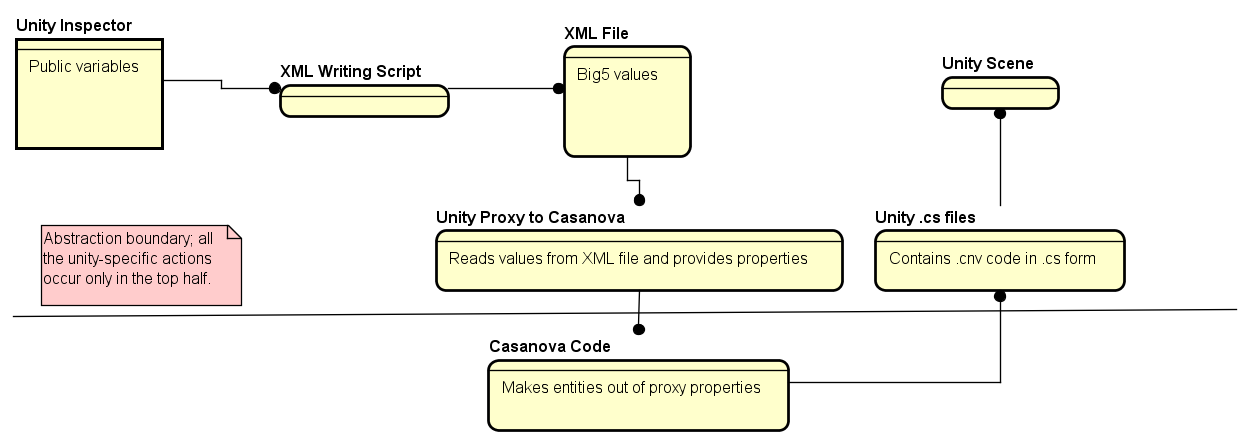
\includegraphics[width=1.4\textwidth]{ER.png}
	\caption{ER-Diagram}
	\label{fig:figure2}
  \end{figure}

  ~\\
  We will most likely provide the big-5 values (or other personality values, more on this later) through an XML file which can be manipulated through the Unity directly inspector. By using an XML file we will be easily able to bring certain personality configurations along on demos and manipulate these configurations from outside of Unity. An important point for us to consider is that the Unity proxies and all other Unity-related pieces of code should not deal with the actual logic of the game; They should only provide an easy interface for Casanova to interact with. By doing this our project will remain relatively independent of Unity, making it easier to use for possible future developers.


  \newpage
  \section{Algorithm structure for a single character}
  In the stages of this project, we will be focusing our attention on having a certain character behave according to his/her personality values and having this character interact with the player accordingly. Characters interacting with other characters is a much more complex subject; we will discuss this in a later chapter. 

  We have identified the most important visible behaviour-characteristics that each avatar should exhibit (almost) regardless of the context of the game in question. There are some exceptions to this rule however, depending on the nature of the game in question. In a relatively static game in which neither player nor npc move around much, like an interrogation-game, movement patterns and walking styles will naturally not be visible. The following list will include examples of each kind of behavior in order to make their distinctions more clear.

  \begin{enumerate}
  	\item Decision-making (Will the character tend to the other NPC who has just fallen over or will I move away?)
  	\item Movement pattern and walking style (Does the NPC move at a steady pace or does he constantly change his walking speed?
  											  Does he walk about confidently or does he slowly wander?) 
  	\item Body Language (What kind of mood does the NPC's body language reflect? Is he standing up proudly or are his shoulders collapsed?)
  	\item Speech (What does the NPC say and with what tone of voice does he say it? What mood does his voice reflect?)
  	\item Facial Expression (Which emotions does the NPC's face reflect? Does his facial expression stay neutral and constant or does it change often and rapidly?)
  \end{enumerate}

  Each of these factors can provide a reasonably visible indication to the player of what kind of personality/emotions the character exhibits. 
  To determine how a certain NPC will display these factors (IE. What the NPC's walking style will be) we will use a personality model. Personality models provide us with a measure of what kind of behavior an NPC who leans to certain sides of a psychological trait would exhibit. 


  \newpage
  \subsection{Change in the behavior of an NPC}
  The behavioral factors of an NPC are changeable and can potentially change for two reasons: Because of the personality of the character itself, or because of certain events that happen to or near the character combined with that characters' personality. Certain personality traits contained in the earlier mentioned personality models, like neuroticism, can cause people to have very variable emotions and extreme emotional reactions to very insignificant events. Within the game, we will likely represent this by having characters with a high neuroticism level change their movement style, body language and facial expression constantly.

  The other way in which we will let our characters behavioral factors change is by subjecting them to certain positive or negative events. Depending on the characters personality, they will respond differently to certain events. An example; NPC 1, who has an egoism value of 100 out of 100 stands next to NPC 2. All of a sudden, NPC 2 lets out a cry of pain and collapses. Because NPC 1 has such a high egoism value, he does not rush to NPC 2's aid: He completely ignores him instead and calmly walks away (An even more cynical reaction might be that NPC 1 starts searching NPC 2 for valuables..).

  If NPC 1 had had a different egoism value, he/she would have reacted differently to this distressing situation. Positive situations will also elicit a certain response depending on the personality values of an NPC. When dance music suddenly starts playing next to a group of NPCs, the extravert ones among them might start to dance, whilst the NPC with very low extraversion scores probably won't dance. 

  Some of the behavioral factors of the NPC's will have to be slightly exagarrated in order for them to be clearly visible to the player and in order for them to be technically viable. Facial expressions in real human beings can be incredible subtle and complex, but emulating exact facial expressions would not only be an incredible technical challenge; it might take extreme player effort in order to actually notice them. Since our focus is still on creating a game, rather than a person simulator, we have prioritized 'playability' over realism.


  \newpage
  \subsection{Our personality models of choice}
   %UITBREIDEM
   For our first prototype of a single avatar, we will be using the Big 5 personality model. This model has several layers of complexity, but for our very first prototype we will be focusing solely on the top level of the Big 5 model. This personality model containts, as the name implies, 5 principle traits by which to measure personality. They are as follows:

   \begin{itemize}
   	\item Extraversion vs. Introversion
   	\item Egoism vs. Altruism
   	\item Thoroughness vs. Chaoticness \footnote{In the original model, the term 'conscientiousness' is used. Since this term did not seem very descriptive to us, we replaced it with 'Thoroughness'.}
   	\item Emotional Stability vs. Neuroticism 
   	\item Openness to new experiences vs . Stubborness (Not supported) \footnote{Item no. 5 is a little harder to implement as very concrete NPC behavior due to it's relevance lying mostly within the psychological growth and gathering of experiences, therefore we will not be using much it in our prototypes.}
   \end{itemize}

    Each of the left-handed personality factors will be given percentage, ranging from 0 to 100 percent. A 100 percent score will mean that the NPC will totally exhibit the given personality factor of the Big 5 model, whilst a 0 percent score will indicate that the NPC will totally exhibit the opposite factor (In the case of Extraversion, this would mean that the NPC is totally introvert). In order to allow the user to create populations of NPC's without having to set each of their values individually, each personality factor will have both a minimum and a maximum percentage. These percentages will indicate between which percentages the scores for this personality factors will range for the NPC population. 

   \newpage
   \subsection{Algorithm structure}
    The algorithm which we will describe here will be responsible for deciding for each character what kind of behavior he/she will display in a given situation. This behavior will consist of a combination of facial expression, body language, speech \footnote{Since we will most likely not have professional voice actors at our disposal, speech will probably consist of text bubbles or even just simple emotes like exclamation marks etc.} movement style and movement pattern and certain decision-making processes. 

    Before the actual algorithm can make decisions on an NPC's behavior, the following will need to be defined:

    \begin{enumerate}
    	\item Define each NPC's personality scores, by choosing a random integer between the minimum and maximum value for each of the four personality factors.
    	\item For each of the personality factors, define behavior consisting combinations of animations, movement patterns, facial expressions, body language and speech. Define multiple behaviors for the extremes of each personality factor (IE. 0 percent extraversion and 100 percent extraversion) and preferably also some in-between behaviors. Define at what end of the spectrum each behavior lies. Note that you might have to define different behaviors for the same personality factors: Behavior for use in events and behavior for use when there are no events happening near the NPC.%LOT OF WORK
    	\item Define a series of events that will be triggered throughout the duration of the game. For each of these events, take all of the four personality factors and give them a threshold value ranging from 0 to 100. The higher this threshold is for a given personality factor, the less likely that an NPC's reaction to this event will be driven by that personality factor.
    \end{enumerate}

    Each frame, there will be a check to see wether the NPC is in the vicinity of an event. If so, the algorithm will do the following:

    \begin{enumerate}
    	\item Get the greatest personality factor of the NPC that is greater than its' equivalent threshold in the event. If there is not a single personality factor of the NPC larger than its' equivalent threshold, stop: The NPC doesn't react to the event.
    	\item Get the event behaviors belonging to the resulting personality factor of step 1, if there is any result. 
    	\item Determine which of the behaviors to trigger using the personality factors' value. (IE. a 100 percent egoism value would warrant a very egoistic behavior, etc.)
    	\item Trigger the behavior.
    \end{enumerate}

    If on the other hand, there is no event within the vicinity of the NPC, every 5 seconds or so the algorithm will do the following:

    \begin{enumerate}
    	\item Sum all of the personality factor values. 
    	\item For each of the personality factors, compute the chance of the behavior relevant to this factor will be triggered: Divide the personality factor value by the result of step 1.
    	\item Order the personality factors by their chance values, starting with the biggest chance. (For instance: Egoism has chance value 30, so gets the first place, Extraversion has chance value 20, so gets the second place, etc.)
    	\item Generate a random number from 0 to 100: Get the personality factor in whose spot the number is. (For instance: If the resulting number is 40, extraversion will be chosen since 0-30 was covered by egoism, and 30-50 was covered by extraversion.)
    	\item Get the personality factor score, NOT the chance value, for the chosen factor and trigger the behavior relevant to that score.
    \end{enumerate}

    %PSEUDOCODE   

	\newpage
	\section{Interaction between NPC's}
	In order to create a realistic feeling for the player, there also needs to be interaction between the different NPC's, rather than just single NPC's displaying behaviors. One way to do this would be in the form of mini-events between NPC's that only occur when NPC's get within a certain range of eachother. 

	%limited to 2 npc's?
	A very basic event that might happen when two NPC's enter each others' personal space is that one of them might try to begin a conversation, if his personality scores \footnote{Within the Big-5 model, Extraversion vs. Introversion and Emotional Stability vs. Neuroticism are the most likely candidates for this task.}. Depending on the personality scores of the other NPC, he/she might accept the invitation. During the conversation, the body language, speech patterns and facial expressions of both NPC's will be governed by their relevant personality scores, like we talked about in the previous section.

	%opzij stappen
	Another simple interaction which would only involve 2 NPC's at a time would be navigation: When an NPC navigates a crowd of other NPC's, they might back away from him or hold their ground, depending once again upon certain of their personality scores. This very simple measure would create a more realistic representation of a crowd or group of actual humans.

	\newpage
	\section{Demonstrating the NPC's}
	 We intend to demonstrate this project by creating a game, or several games, in which player NPC interaction and NPC personalities will be key concepts. 

  	%Hoe gaat de demo eruitzien, welke events kiezen we uit
  	%Big5 model uitwerking als bijlage toevoegen

\end{document}